\nxsection{Le R\^ole ''Manager''}\label{sec:utilisateurs-lepatron}
\index{patron}
\index{Manager}

La figure~\ref{fig:yeren-fenetre-patron} illustre la fen\^etre
d'acceuil d'un utilisateur avec le \role \manager, 
apr\`es qu'il se soit enregistr\'e dans \yeren.\\

\begin{figure}[!htbp]
\centering
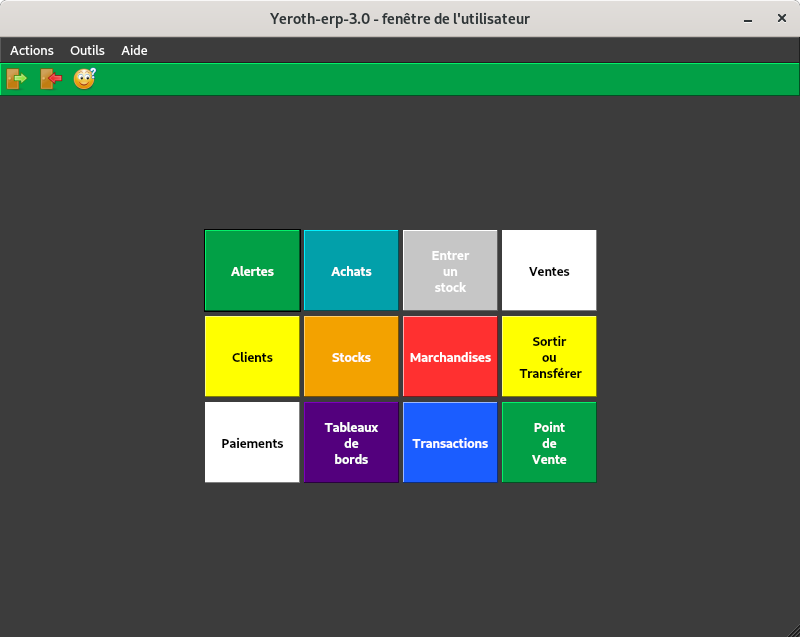
\includegraphics[scale=0.63]{images/yeroth-fenetre-manager.png}
\caption{La fen\^etre d'acceuil d'un \manager}
\label{fig:yeren-fenetre-patron}
\end{figure}

Un utilisateur de \yeren avec le \role \manager a acc\`es
aux fonctionnalit\'es suivantes:

\begin{enumerate}[1)]
	\item administration (voir chapitre~\ref{chap:administration-logiciel})
	\item gestion des achats (voir chapitre~\ref{chap:gestion-des-achats})
	\item gestion des clients (voir chapitre~\ref{chap:gestion-des-clients})
	\item gestion des stocks (voir chapitre~\ref{chap:gestion-stocks})
	\item gestion des ventes (voir chapitre~\ref{chap:vente})	
	\item mouvements de stocks (voir chapitre~\ref{chap:mouvements-de-stocks})
	\item point de vente (voir chapitre~\ref{chap:vendre})	
	\item syst\`eme d'alertes (voir chapitre~\ref{chap:systeme-dalertes})
	\item tableaux de bords (voir chapitre~\ref{chap:tableaux-de-bords}).\\
\end{enumerate}